\documentclass[twocolumn, 10pt, times, letterpaper]{article}
\usepackage[margin=1in]{geometry} %one inch margins
\usepackage{pslatex}
\usepackage{mathptmx}
\usepackage{listings}
\usepackage{achicago}
%\usepackage{fleqn} %sets equation to left
\usepackage{amsmath, amssymb}
%\usepackage{fancyhdr}
\usepackage{epsfig}
%\usepackage{pstricks,pst-node,pst-tree,pst-plot}
\usepackage{graphicx}
\usepackage{vmargin}
\usepackage{url}
\usepackage{tabularx}
% \usepackage{ccaption}
\usepackage{mathtools}  % for special symbols such as :=
\usepackage{xspace}
\usepackage{todonotes}
\usepackage{tikz}
\usepackage[utf8]{inputenc}
\usepackage{pgfplots} 
\usepackage{pgfgantt}
\usepackage{pdflscape}
\pgfplotsset{compat=newest} 
\pgfplotsset{plot coordinates/math parser=false}
\newlength\fwidth
\newlength\hwidth

\usepackage{lastpage} % for the number of the last page in the document
\usepackage{fancyhdr}

%%%%%%%%%%%%%%%%% Macros used in the paper %%%%%%%%%%%%%%%%%%%%

\newcommand{\tX}{\mathsf{X}}
\newcommand{\tY}{\mathsf{Y}}
\newcommand{\tZ}{\mathsf{Z}}
\newcommand{\tP}{\mathsf{P}}
\newcommand{\tT}{\mathsf{T}}
\newcommand{\D}{\mathcal{D}}

% Auto-regressive vector
\newcommand{\arvec}[1]{\ensuremath{\boldsymbol{#1}}}  % ^{\leftarrow}
\def\Pbatt{\ensuremath{b}}
\def\Ptotal{\ensuremath{p}}
\def\Pbmax{\ensuremath{\Pbatt_{\mathrm{max}}}}
\def\Pbmin{\ensuremath{\Pbatt_{\mathrm{min}}}}
\def\SOCmax{\ensuremath{s_{\mathrm{max}}}}
\def\SOCmin{\ensuremath{s_{\mathrm{min}}}}

\newcommand{\GaussianDist}[2]{\ensuremath{\operatorname*{\mathcal{N}}\left(#1, #2\right)}}  % Gaussian distribution given mean and variance
\newcommand{\GaussianDistSmall}[2]{\ensuremath{\operatorname*{\mathcal{N}}(#1, #2)}}  % Gaussian distribution given mean and variance

% Typeset predicted variables. Usage:
% \predict{k}{u} --> predicted u at k | t
% \predict[\tau]{k}{u} --> predicted u at k | \tau
\newcommand{\predict}[3][t]{\ensuremath{#3}_{#2 | #1}}

\newcommand{\sigmamax}[1][0]{\ensuremath{\overbar{\sigma}_{#1}}}

\newcommand{\eg}{e.g.,\xspace}
\newcommand{\ie}{i.e.,\xspace}
\newcommand{\etc}{etc.\xspace}
\newcommand{\cf}{cf.~}

% Some commonly used math functions/operators
\DeclareMathOperator*{\argmin}{arg\,min}
\DeclareMathOperator*{\argmax}{arg\,max}
\DeclareMathOperator*{\minimize}{minimize}
\DeclareMathOperator*{\maximize}{maximize}
\DeclareMathOperator{\sgn}{sgn}  % the signum/sign function

\newcommand{\RR}{\mathbb{R}\xspace}  % Real set
\newcommand{\NN}{\mathbb{N}\xspace}  % Natural number set
\newcommand{\QQ}{\mathbb{Q}\xspace}  % Rational number set
\newcommand{\CC}{\mathbb{C}\xspace}  % Complex number set
\newcommand{\ZZ}{\mathbb{Z}\xspace}  % Integer number set
\newcommand{\EE}{\mathbb{E}\xspace}  % Expectation
\newcommand{\PP}{\mathbb{P}\xspace}  % Probability
\newcommand{\BB}{\mathbb{B}\xspace}  % Logic set {true, false}


% -------------------------------------------------------------------
% Different font in captions
% from http://dcwww.camp.dtu.dk/~schiotz/comp/LatexTips/LatexTips.html
\newcommand{\captionfonts}{\it}
\makeatletter  % Allow the use of @ in command names
\long\def\@makecaption#1#2{%
  \vskip\abovecaptionskip
  \sbox\@tempboxa{{\captionfonts #1: #2}}%
  \ifdim \wd\@tempboxa >\hsize
    {\captionfonts #1: #2\par}
  \else
    \hbox to\hsize{\hfil\box\@tempboxa\hfil}%
  \fi
  \vskip\belowcaptionskip}
\makeatother   % Cancel the effect of \makeatletter
% -------------------------------------------------------------------

% PDF Links --------------------------------------------------------
%% \usepackage[ps2pdf,colorlinks]{hyperref}
%%  \hypersetup{backref, %
%%    colorlinks=true, %
%%    linkcolor=black, %
%%    anchorcolor=black, %
%%    citecolor=black, %
%%    filecolor=black, % Color for URLs which open local files.
%%    menucolor=black, % Color for Acrobat menu items.
%%    pagecolor=black, % Color for links to other pages.
%%    urlcolor=black, %
%%    pdftitle={}, %
%%    pdfauthor={}, %
%%    pdfsubject={}, %
%%    pdfkeywords={}%
%%  }
% Fuzz -------------------------------------------------------------------
\hfuzz4pt % Don't bother to report over-full boxes if over-edge is < 2pt
\vfuzz=\hfuzz
% THEOREM Environments ---------------------------------------------------
\newtheorem{definition}{Definition}
\newtheorem{assumption}{Assumption}
\newtheorem{theorem}{Theorem}
\newtheorem{lemma}{Lemma}
\newtheorem{corollary}{Corollary}
\newtheorem{proposition}{Proposition}
\newtheorem{algorithm}[theorem]{Algorithm}
\newcommand{\rbox}{ \qed }

\renewcommand{\Re}{{\mathbb R}}
\newcommand{\Na}{{\mathbb N}}
\newcommand{\Z}{{\mathbb Z}}

% Depth of table of contents -----------------------------------------
\setcounter{tocdepth}{2}

%QED box, from the TeXbook, p. 106. ----------------------------------
\newcommand\qed{{\unskip\nobreak\hfil\penalty50\hskip2em\vadjust{}
    \nobreak\hfil$\Box$\parfillskip=0pt\finalhyphendemerits=0\par}}


% Line spacing -----------------------------------------------------------
\newlength{\defbaselineskip}
\setlength{\defbaselineskip}{\baselineskip}
\newcommand{\setlinespacing}[1]%
           {\setlength{\baselineskip}{#1 \defbaselineskip}}
\newcommand{\doublespacing}{\setlength{\baselineskip}
                           {2.0 \defbaselineskip}}
\newcommand{\singlespacing}{\setlength{\baselineskip}{\defbaselineskip}}
\newcommand{\onehalfspacing}{\setlength{\baselineskip}
                           {1.5 \defbaselineskip}}

\hyphenation{TRNSYS}

% Page layout ------------------------------------------------------------
% see LaTeX Companion, p. 83ff
\setlength{\hoffset}{-37 mm}
\setlength{\topmargin}{0mm}%
\setlength{\textwidth}{16.8cm}
\setlength{\textheight}{22.7cm}
\setlength{\headheight}{31.75mm}
\setlength{\headsep}{12pt}
%\setlength{\footheight}{12pt}
\setlength{\footskip}{12pt}
\setlength{\parindent}{0pt}

%\setlength{\columnsep}{8mm}
\setlength{\columnsep}{0.25in}
\setcounter{secnumdepth}{-2} % to avoid numbering
%\setlength{\mathindent}{0mm}

% -------------------------------------------------------------------------
% Section headings
% p. 27
\makeatletter
\renewcommand{\section}{\@startsection
	{section}%            %the name
	{0}%                  %the level
	{0mm}%                %the indent
	{6pt}%               %the beforeskip
	{3pt}%                %the afterskip
	{\noindent \fontsize{12}{14}\selectfont \underline}}  %the style
%   {\noindent \large \sc \underline}}  %the style

\renewcommand{\subsection}{\@startsection
	{subsection}%            %the name
	{1}%                  %the level
	{0mm}%              t  %the indent
	{6pt}%               %the beforeskip
	{3pt}%                %the afterskip
	{\noindent \fontsize{10}{12}\selectfont \bf}}  %the style
%   {\noindent \bf}}  %the style
\makeatother

% Make capitalized reference header for IBPSA
\renewcommand{\refname}{REFERENCES}

\newcommand{\authorfont}{\fontsize{12}{14}\selectfont}
\newcommand{\titlefont}{\fontsize{12}{14}\selectfont \bf}
% -------------------------------------------------------------------------
\pagestyle{empty}

% -------------------------------------------------------------------------
% Contents ----------------------------------------------------------------
\begin{document}
\fancypagestyle{empty}{%
  \fancyhf{}% Clear header/footer
  \renewcommand{\headrulewidth}{1.5pt}
  \fancyhead[L]{
\includegraphics [width=1.5in] {images/logo_new.jpg}}
% conference logo
  \fancyhead[R]{2018 Building Performance Modeling Conference and \\ SimBuild co-organized by ASHRAE and IBPSA-USA \\ Chicago, IL \\ September 26-28, 2018}% header text
}

%\onehalfspacing
\bibliographystyle{achicago}
\renewcommand{\SCduplicate}[1]{#1}
\date{}
\title{\vspace{-9mm} \titlefont %
	DIGITAL TWINS FOR EFFICIENT MODELING AND CONTROL OF BUILDINGS
	}
%\author{%
%\authorfont{John Modeller$^1$, Jane Simulator$^2$, and Another Author$^3$}\\
%\authorfont{$^1$Technical University, Cambridge, MA}\\
%\authorfont{$^2$Another Institution, Some City, Some Country}\\
%\authorfont{The names and affiliations SHOULD NOT be included in the draft submitted for review.}\\
%\authorfont{The header consists of 10 lines with exactly 14 point spacing.}\\
%\authorfont{The line numbers are for information only. The last line below should be left blank.}\\
%\authorfont{~}\\ % used to add blank lines
%\vspace{-14mm}
%}
\maketitle
\thispagestyle{empty}

% --------------------------------------------------------
\section{ABSTRACT}

We develop an integrated solution for incorporating ``digital twins” of real buildings into existing SCADA systems, which enables real-time prediction and advanced control. 
These digital twins are either EnergyPlus (E+) or data-driven (D+) building models, whose input and output variables are mapped to analogous real building OPC tags and track the real-time operation of the building.
An E+ digital twin can be used to provide predictions of the building’s performance in different weather, usage, and energy pricing scenarios, which allows for accurate assessment of different control strategies. 
However, it is not suitable for optimization and predictive control due to its complexity. 
We develop scalable D+ digital twin based on Gaussian Processes (GP) for accurate prediction and advanced control. 
A D+ digital twin is much easier, faster, and less expensive to train than developing and tuning an E+ model, while still providing accurate power forecasts and being suitable for control. 
Data-driven Model Predictive Control (MPC) optimizes control inputs of the predictive D+ model for energy curtailment with thermal comfort guarantees in demand response applications.
The MPC controller is integrated into the SCADA environment, demonstrating real-time in-the-loop control of D+ digital twins.

%%% Local Variables:
%%% mode: latex
%%% TeX-master: "main"
%%% End:


% --------------------------------------------------------
\section{INTRODUCTION}

% --------------------------------------------------------
\section{DATA ACQUISITION \& COMMUNICATION}

In a building automation system, a Supervisory Control and Data Acquisition (SCADA) system is commonly used by the operators to manage individual buildings or a campus of buildings. 
It interfaces directly with building sensors and controllers through open source protocols like BACNet or OPC. 
SCADA software also provides a dashboard interface for the operators to view live or historical data feeds from the sensors and an easy way for operators to change control setpoints remotely. 
Additionally, it may also offer a Historian database to store historical data values for future reference or data analysis.
See Figure \ref{F:intro} for an illustration of a typical SCADA system.

There are two main limiting factors in bridging digital twins with existing SCADA software.
First, most SCADA software are self-contained and the features are limited to those provided by the vendor.
Building operators cannot view the results from E+/D+ models on the same SCADA software used for real-time monitoring because it is not clear how we can communicate between the E+/D+ models and existing SCADA software to acquire the data tags required by E+/D+ models for simulation and control, and to show the generated results on the dashboards.
Second, if the digital twin is an E+ model, we need an external library like MLE+ \cite{bernaletal12mti} to design a controller in a scripting language such as MATLAB.
This is because EnergyPlus only allows to manually code rule-based control strategies.
Since Python is a popular programming language for data science and machine learning, we need an alternative to MLE+ for Python. 

In this work, we use the open interface OPC to connect EnergyPlus with any existing SCADA softwarethat supports OPC for real-time data communication. 
We call this EnergyPlus-OPC bridge.
By representing inputs to and outputs from EnergyPlus as OPC tag structures, we make the integration into existing SCADA software significantly easier since the simulated building will appear as a real building to the SCADA software.
Furthermore, since our machine learning models are written in Python, we develop a library to interface Python and EnergyPlus called \texttt{pyEP}, an equivalent to MLE+ for Python.
We show how this library allows for intelligent control of buildings using D+ models and testing on E+ models.
The transition from testing on E+ models to testing on real buildings can be made seamlessly through the SCADA system.

% In summary, E+ models cannot be used for designing advanced controllers like MPC. 
% But an interface like MLE+ (MATLAB) and \texttt{pyEP} (Python) allows the users to test manual control strategies more conveniently.
% On the other hand, as we show in Section \ref{S:dpc}, D+ models, are suitable for MPC.
% In the examples that will follow, we will test a controller based on a D+ model on an E+ model as a plant (substitute for a real building).
% This setup is shown in Figure \ref{F:control}.
% The EnergyPlus-OPC bridge allows us to interface the E+/D+ models to the SCADA software and enables to study a closed-loop response of this building.
% Once the optimal setpoints are obtained from MPC, and the corresponding digital twin response behavior can be viewed in real time in a commercial SCADA dashboard.

The case studies presented later in this paper use the setup shown in Figure \ref{F:control}, in which a data-driven controller based on a D+ model acts on an E+ model as a plant.
The EnergyPlus-OPC bridge allows us to interface an E+/D+ model to the SCADA software for real-time monitoring and closed-loop control of the building.
The setpoints obtained from the controller and the corresponding responses from the digital twin can be viewed in real time in a commercial SCADA dashboard.

\begin{figure}[t]
	\centering
	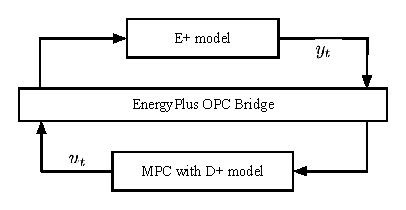
\includegraphics[width=0.4\textwidth]{images/control.eps}
	\caption{The MPC controller runs in Python using the D+ models and applies the optimal inputs to the E+ model. The communication is made possible using the \texttt{pyEP} library and the OPC connection.}
	\label{F:control}
\end{figure}

\subsubsection{EnergyPlus-OPC Bridge}

Our EnergyPlus-OPC bridge provides the EnergyPlus input and output variables as OPC tags to be read by any OPC client.
The user is able to configure the simulation for any number or type of buildings and can run each individually on different schedules.
To see the simulation in progress, the operators only need to view the tag, as they would for any other data source.
By writing to one of the input tags, the operators can change the input setpoints to EnergyPlus and see the response of the building.
For more advanced controls of the building, the operators can use our MPC controller based on D+ models.
The service supports the running of multiple EnergyPlus instances, creating a campus of isolated buildings.
The buildings are simulated synchronously, so that their simulations are always kept at the same time. % sequentially, but kept at the same time, so that the first building only advances a time step when all other buildings are at the same time.
This capability can be useful when looking at aggregate power consumption and synthesizing control strategies involving multiple-building curtailment.
For communication between EnergyPlus and Python we use \texttt{pyEP}.

\subsection{pyEP: A Python EnergyPlus Interface}

Currently, EnergyPlus supports external programs through the Building Controls Virtual Testbed (BCVTB), built on top of Ptolemy II, and the Functional Mockup Interface (FMI) standard. 
Using BCVTB, the users can couple and define data flows between various modeling and simulation programs, such as TRNSYS or Simulink. 
These simulation environments, while comprehensive, are still constrained by the capabilities of the software. 
MLE+ provides a solution to this problem, allowing the end-users to directly control the progress of an EnergyPlus simulation by writing MATLAB code. 
In recent years, Python has become a popular language for data science and machine learning, in academia and especially in industry. % but   with many advanced open-source libraries like TensorFlow \cite{Abadid} and Scikit-learn \cite{Pedregosa2011} being used widely in industry and academia.
The \texttt{pyEP} library connects the myriad of Python libraries with existing technologies in the building modeling and simulation communities.
For example, in our case studies depicted in Figure \ref{F:control}, we obtain data from EnergyPlus to learn D+ models, which are used for synthesizing building control strategies, then evaluate these strategies in closed-loop simulation with EnergyPlus.
These steps are made possible by \texttt{pyEP}.
%This communication has been made possible with the \texttt{pyEP} library.

The \texttt{pyEP} library is designed to be lightweight and flexible. 
The core class is \texttt{ep\_process}, which provides simple read and write capabilities with EnergyPlus. 
Each \texttt{ep\_process} instance corresponds to one EnergyPlus building, and is independent of all other \texttt{ep\_process} instances. 
% This means that \(\mathtt{idf}\) files (format specific to EnergyPlus) built for different EnergyPlus versions, or buildings with different weather files, can be run together in a campus-like co-simulation.
This allows for multiple EnergyPlus models being run together in a campus-like co-simulation. 
An example using the Department of Energy (DoE) provided LargeOffice building model is included in the installation. 
For an EnergyPlus IDF model file to be used with \texttt{pyEP}, it must have the \texttt{ExternalInterface} configured, as well as an associated \texttt{variables.cfg}, specifying the inputs and outputs to the \texttt{ExternalInterface}.
\texttt{pyEP} is available on the Python Package Index (PyPI) and can be installed with the command \verb|pip install pyEP|.
Its documentation can be found at \url{https://github.com/mlab-upenn/pyEP}.

\subsubsection{System Architecture}

\todo[inline]{May include a picture here, and reduce the text below.}

The EnergyPlus-OPC bridge service requires two processes to start and control a simulation. 
The first is the bridge itself, which can be started once and left in the background indefinitely. 
The second is a controller, which determines which setpoints to write to the bridge at what time during the simulation. 
The role of the bridge is to handle communication between EnergyPlus and the OPC server. 
The role of the controller is to control the inputs at every time step of the EnergyPlus co-simulation.
At time step $t$, the bridge first writes the outputs from EnergyPlus at the previous time step $t-1$. 
The controller then reads the outputs and uses them to determine the next set of inputs to write to the EnergyPlus input tags. 
%For a controller running on a fixed schedule, it would use the simulation time to determine what setpoints to write. 
%A more energy-savings focused controller might use the current power consumption to determine if a curtailment strategy should be implemented instead. 
After the controller writes them to the input OPC tags, the bridge reads them and passes them into EnergyPlus. 
The same process follows for the next building, until all have been incremented forward by one time step.
The communication protocol ensures that every input and output are read to the correct EnergyPlus building, and that delays in the network communications do not cause the controller and bridge to become out-of-sync with each other. 
The exchange of information is not real-time dependent, so human operators can change the inputs time step by time step at any pace. 
The controller can also preemptively stop a simulation by terminating the controller process. 
Changes to a prescribed schedule can also be made, and the simulation restarted again without needing to restart the bridge process. 
This allows for easier changes and less time overhead between simulation runs.
Specific syntax can be found in the documentation. 
The bridge should only be restarted if different EnergyPlus buildings need to be used.

This bridge-controller design provides great flexibility in how the user can make use of EnergyPlus. 
Users can freely modify the controller to customize the simulation parameters. 
A simple schedule based controller monitoring power consumption can be made with basic knowledge of Python. 
Alternatively, more complex model-based controllers like MPC as in Section \ref{S:dpc} can also be implemented and evaluated.
Two example controllers are included in the \texttt{pyEP} library. 
The first controller implements a setpoint schedule in Python and shows how to read/write from the controller to EnergyPlus. 
The second controller implements a setpoint schedule based on a formatted csv file. 
% No knowledge of Python is needed to edit and run a custom setpoint schedule.

\subsubsection{Requirements}

The provided controllers use the OpenOPC library to connect to an OPC server, but other methodologies may be used if the communications paradigm is followed. See \texttt{pyEP} documentation for more details.
Additionally, the free Matrikon OPC Server Simulator is used as the default server.
Included with \texttt{pyEP} is a server configuration XML generator that automatically creates the correct OPC Tree Tag structure for the Matrikon Server. 
The \texttt{pyEP} core module, linking EnergyPlus to Python, is supported for Python 2.7 and 3.x, while the EnergyPlus-OPC bridge requires Python 2.7.

%%% Local Variables:
%%% mode: latex
%%% TeX-master: "main"
%%% End:


% --------------------------------------------------------
\section{MODELING WITH GAUSSIAN PROCESSES}
\label{S:gp}

As mentioned earlier, conventional building modeling methods based on first principles are time-consuming and cost-prohibitive.
Data-driven modeling approaches, based on machine learning techniques, have been shown to be fast, economical, and accurate alternatives.
This section presents a building modeling approach with Gaussian Process (GP), starting with a brief introduction to GP and its application in controls.

\subsection{Introduction to Gaussian Process}
\label{sec:gp:gp-intro}

\begin{definition}%[\cite{Rasmussen2006}]
A Gaussian Process is a collection of random variables, any finite number of which have a joint Gaussian distribution.
\end{definition}
%
Consider an unknown function \(f: \RR^n \mapsto \RR\) with noisy observations \(y = f(x) + \GaussianDist{0}{\sigma_n^2}\).
A GP of \(y\) is specified by its mean function \(\mu(x)\) and covariance function \(k(x,x')\),
\begin{align}
\label{E:gp:prior}
\mu(x; \theta) &= \EE [f(x)] \\
k(x,x'; \theta) &= \EE [(f(x)\!-\!\mu(x)) (f(x') \!-\! \mu(x'))] + \sigma_n^2 \delta(x,x') \nonumber
\end{align}
where \(\delta(x,x')\) is the Kronecker delta function.
These functions are parameterized by the hyperparameter vector \(\theta\).
The covariance function \(k(x,x')\) specifies how the outputs at \(x\) and \(x'\) are correlated.
In other words, a GP model of \(y\) specifies the relationship between the input variables, through the covariance function, rather than a fixed structural input--output relationship from $x$ to $y$.

Given the regression vectors \(X = [x_1, \dots, x_N]^T\) and their corresponding observed outputs \(Y = [y_1, \dots, y_N]^T\), the distribution of the output \(y_\star\) corresponding to a new input vector \(x_\star\) is a Gaussian distribution \(\GaussianDist{\bar{y}_\star}{\sigma_\star^2}\),
\begin{subequations}
\label{E:gp-regression}
\begin{align}
\bar{y}_\star &= g_{\mathrm{m}} (x_{\star}) \coloneqq \mu(x_\star) + K_\star K^{-1} (Y - \mu(X))\\
\sigma_\star^2 &= g_{\mathrm{v}} (x_{\star}) \coloneqq K_{\star \star} - K_\star K^{-1} K_\star^T \text,
\end{align}
\end{subequations}
where \(K_\star = [k(x_\star, x_1), \dots, k(x_\star, x_N)]\), \(K_{\star \star} = k(x_\star, x_\star)\), and $K$ is the covariance matrix with elements \(K_{ij} = k(x_i, x_j)\).
The hyperparameters $\theta$ can be learned by maximizing the likelihood: \(\argmax_\theta \Pr(Y \vert X, \theta)\).
%It is therefore highly flexible and can capture complex behavior with fewer parameters.
An example of GP prior and posterior is shown in Fig.~\ref{F:gp:prior:posterior}. %, where a constant mean function and a covariance function consisting of a squared exponential kernel and a rational quadratic kernel are used.


\begin{figure}[!tb]
  \centering
  \setlength\fwidth{\columnwidth}
  \setlength\hwidth{0.5\fwidth}
  \resizebox{\columnwidth}{!}{% This file was created by matlab2tikz.
%
%The latest updates can be retrieved from
%  http://www.mathworks.com/matlabcentral/fileexchange/22022-matlab2tikz-matlab2tikz
%where you can also make suggestions and rate matlab2tikz.
%
\definecolor{mycolor1}{rgb}{0.97647,0.89804,1.00000}%
%
\begin{tikzpicture}

\begin{axis}[%
width=\fwidth,
height=0.982\hwidth,
at={(0\fwidth,0\hwidth)},
scale only axis,
xmin=1,
xmax=48,
xtick={8,16,24,32,40},
xticklabels={{2am},{4am},{6am},{8am},{10am}},
ymin=13.8495974547768,
ymax=404.39922079824,
ylabel style={font=\color{white!15!black}},
ylabel={power [kW]},
axis background/.style={fill=white},
legend style={at={(0.5,1.03)}, anchor=south, legend columns=4, legend cell align=left, align=left, fill=none, draw=none},
xlabel style={font=\footnotesize},ylabel style={font=\footnotesize},legend style={font=\footnotesize},ticklabel style={font=\footnotesize},ylabel shift = -5 pt,xlabel shift = -5 pt,
]

\addplot[area legend, draw=white!75!gray, fill=white!75!gray]
table[row sep=crcr] {%
x	y\\
1	386.646965191719\\
2	386.646965191719\\
3	386.646965191719\\
4	386.646965191719\\
5	386.646965191719\\
6	386.646965191719\\
7	386.646965191719\\
8	386.646965191719\\
9	386.646965191719\\
10	386.646965191719\\
11	386.646965191719\\
12	386.646965191719\\
13	386.646965191719\\
14	386.646965191719\\
15	386.646965191719\\
16	386.646965191719\\
17	386.646965191719\\
18	386.646965191719\\
19	386.646965191719\\
20	386.646965191719\\
21	386.646965191719\\
22	386.646965191719\\
23	386.646965191719\\
24	386.646965191719\\
25	386.646965191719\\
26	386.646965191719\\
27	386.646965191719\\
28	386.646965191719\\
29	386.646965191719\\
30	386.646965191719\\
31	386.646965191719\\
32	386.646965191719\\
33	386.646965191719\\
34	386.646965191719\\
35	386.646965191719\\
36	386.646965191719\\
37	386.646965191719\\
38	386.646965191719\\
39	386.646965191719\\
40	386.646965191719\\
41	386.646965191719\\
42	386.646965191719\\
43	386.646965191719\\
44	386.646965191719\\
45	386.646965191719\\
46	386.646965191719\\
47	386.646965191719\\
48	386.646965191719\\
48	31.6018530612979\\
47	31.6018530612979\\
46	31.6018530612979\\
45	31.6018530612979\\
44	31.6018530612979\\
43	31.6018530612979\\
42	31.6018530612979\\
41	31.6018530612979\\
40	31.6018530612979\\
39	31.6018530612979\\
38	31.6018530612979\\
37	31.6018530612979\\
36	31.6018530612979\\
35	31.6018530612979\\
34	31.6018530612979\\
33	31.6018530612979\\
32	31.6018530612979\\
31	31.6018530612979\\
30	31.6018530612979\\
29	31.6018530612979\\
28	31.6018530612979\\
27	31.6018530612979\\
26	31.6018530612979\\
25	31.6018530612979\\
24	31.6018530612979\\
23	31.6018530612979\\
22	31.6018530612979\\
21	31.6018530612979\\
20	31.6018530612979\\
19	31.6018530612979\\
18	31.6018530612979\\
17	31.6018530612979\\
16	31.6018530612979\\
15	31.6018530612979\\
14	31.6018530612979\\
13	31.6018530612979\\
12	31.6018530612979\\
11	31.6018530612979\\
10	31.6018530612979\\
9	31.6018530612979\\
8	31.6018530612979\\
7	31.6018530612979\\
6	31.6018530612979\\
5	31.6018530612979\\
4	31.6018530612979\\
3	31.6018530612979\\
2	31.6018530612979\\
1	31.6018530612979\\
}--cycle;
\addlegendentry{$\text{prior }\mu\text{ }\pm\text{ 2}\sigma$}

\addplot [color=black, dashed, line width=1.0pt]
  table[row sep=crcr]{%
1	209.124409126508\\
48	209.124409126508\\
};
\addlegendentry{$\text{prior }\mu$}


\addplot[area legend, draw=mycolor1, fill=mycolor1]
table[row sep=crcr] {%
x	y\\
1	154.709201629968\\
2	166.075918612389\\
3	139.2395727394\\
4	150.627198219011\\
5	156.562639738461\\
6	172.537252098066\\
7	149.736958849622\\
8	122.449211106838\\
9	137.147704214366\\
10	127.377735086393\\
11	143.923100614629\\
12	154.245932548526\\
13	122.463825041785\\
14	172.450813790158\\
15	162.394161326987\\
16	153.102756456198\\
17	130.944901359138\\
18	218.014957344162\\
19	247.60829556031\\
20	218.774750045423\\
21	232.998363083984\\
22	270.795112821555\\
23	268.724584385649\\
24	290.95948553084\\
25	300.682967077219\\
26	294.875735172657\\
27	314.757769779285\\
28	313.247180951257\\
29	347.323672820772\\
30	296.05671917331\\
31	301.042057704437\\
32	267.702473452336\\
33	273.088289651178\\
34	209.312427630456\\
35	216.802255898329\\
36	268.633216087559\\
37	228.988631430966\\
38	213.423993131178\\
39	183.181633964876\\
40	201.306696759562\\
41	204.566034839882\\
42	238.727065874924\\
43	255.945408503762\\
44	253.536624332962\\
45	272.918841238678\\
46	229.369289663929\\
47	227.109791028515\\
48	192.638566318614\\
48	156.024126508636\\
47	190.753621171366\\
46	193.032780488085\\
45	236.383047496946\\
44	215.860169346718\\
43	219.236377026459\\
42	202.616050681686\\
41	168.172667959549\\
40	165.052675911654\\
39	145.557971092335\\
38	176.467689053364\\
37	191.914942913949\\
36	231.696582339222\\
35	179.351228779518\\
34	173.400552712333\\
33	237.031606471281\\
32	230.183454657379\\
31	263.557792224223\\
30	258.261638782427\\
29	308.397338208832\\
28	274.619563878076\\
27	276.795039204419\\
26	255.661011500426\\
25	261.710731210065\\
24	252.646146479488\\
23	231.178525931647\\
22	234.338683404564\\
21	195.569106888561\\
20	180.844093749074\\
19	210.380218922248\\
18	182.080400287927\\
17	95.6282421712857\\
16	117.359884257066\\
15	126.407916512676\\
14	136.673795119128\\
13	86.5352281989955\\
12	117.899804518827\\
11	106.897592885672\\
10	89.6440805991176\\
9	99.1791317367729\\
8	85.6454991550155\\
7	112.808368940314\\
6	136.547182527759\\
5	120.805709082496\\
4	113.744125160121\\
3	102.833336478683\\
2	129.510389380878\\
1	118.072007567044\\
}--cycle;
\addlegendentry{$\text{posterior }\mu\text{ }\pm\text{ 2}\sigma$}

\addplot [color=red]
  table[row sep=crcr]{%
1	136.390604598506\\
2	147.793153996633\\
3	121.036454609042\\
4	132.185661689566\\
5	138.684174410479\\
6	154.542217312913\\
7	131.272663894968\\
8	104.047355130927\\
9	118.163417975569\\
10	108.510907842755\\
11	125.410346750151\\
12	136.072868533677\\
13	104.49952662039\\
14	154.562304454643\\
15	144.401038919831\\
16	135.231320356632\\
17	113.286571765212\\
18	200.047678816045\\
19	228.994257241279\\
20	199.809421897248\\
21	214.283734986272\\
22	252.566898113059\\
23	249.951555158648\\
24	271.802816005164\\
25	281.196849143642\\
26	275.268373336542\\
27	295.776404491852\\
28	293.933372414666\\
29	327.860505514802\\
30	277.159178977869\\
31	282.29992496433\\
32	248.942964054857\\
33	255.059948061229\\
34	191.356490171394\\
35	198.076742338924\\
36	250.164899213391\\
37	210.451787172458\\
38	194.945841092271\\
39	164.369802528606\\
40	183.179686335608\\
41	186.369351399715\\
42	220.671558278305\\
43	237.590892765111\\
44	234.69839683984\\
45	254.650944367812\\
46	211.201035076007\\
47	208.931706099941\\
48	174.331346413625\\
};
\addlegendentry{$\text{posterior }\mu$}

\end{axis}
\end{tikzpicture}%}
  \caption{Example of priors calculated using \eqref{E:gp:prior} and
    posteriors using \eqref{E:gp-regression} for predicting power
    consumption of a building for \(12\) hrs. Initially the mean is
    constant because \(\mu(x)\) is constant, and we observe a high
    variance. The posterior agrees with the actual power consumption
    with high confidence.}
  \label{F:gp:prior:posterior}
\end{figure}

GP models have several advantages over other machine learning models, that make them more suitable for identification of dynamical systems.
\begin{enumerate}
\item GPs provide predictive variances, which carry uncertainty information of the predictions. The full predictive distribution, which includes both the mean and variance, can be used in a meaningful way, \eg to estimate a 95\% confidence bound for the prediction.
\item GPs work well with small data sets due to its stochastic nature, which is generally useful for any modeling application.
\item GPs allow incorporating domain knowledge of the system %behavior
  into the model to improve its accuracy, by defining priors on the hyperparameters or using a particular structure of the covariance function.
\end{enumerate}

More details on GPs and their applications can be found in \cite{Rasmussen2006}.

\subsection{Gaussian Processes for Dynamical Systems}
\label{SS:intro-gp:control}

Consider a nonlinear dynamical system with control input \(u\), exogenous disturbance input \(w\), and output \(y\).
At a current time step $t$, time-delayed input and output signals are called \emph{autoregressive}, for example: $y_{t-1}, u_{t-1}, w_{t-1}$.
By feeding autoregressive inputs and outputs to a GP as regressors, we can model the dynamic behavior of the system \cite{Kocijan2016}.
Specifically, the regressor vector $x_{t}$ at time step $t$ would be
\begin{equation*}
x_{t}\!=\![y_{t-l}, \dots, y_{t-1}, u_{t-m}, \dots, u_t, w_{t-p}, \dots, w_{t-1}, w_t] \text.
\end{equation*}
where \(l\), \(m\), and \(p\) are respectively the lags for autoregressive outputs, control inputs, and disturbances.
Note that \(u_t\) and \(w_t\) are the current control and disturbance inputs.
The dynamical GP
\begin{math}
y_{t} = f(x_t)
\end{math}
can then be trained from data in the same way as any other GPs.

In a multistep simulation of a dynamical GP, the autoregressive outputs fed to the model beyond the first step are random variables, resulting in more and more complex output distributions as we go further.
Therefore, it involves uncertainty propagation through the model, which would complicate the computation of the model significantly.
\cite{nghiemetal16gp} showed that a simple simulation method called \emph{zero-variance method}, which replaces the autoregressive signals with their corresponding expected values, could achieve sufficient prediction accuracy while benefitting from computational simplicity.
In this paper, the zero-variance method was selected for predicting future outputs in optimization formulations.


\subsection{Modeling Building's Power Demand with GP}
\label{sec:gp:bldg-modeling}

Our aim is to model a building's power demand behavior from data that can be measured directly from installed sensors like thermostats, multimeters and weather forecasts.
The following feature variables are considered:
\begin{itemize}
\item \textit{Weather variables \(d^w\):} such as outside temperature and humidity, which are derived from historical weather data.
\item \textit{Proxy variables \(d^p\):} such as time of day and day of week, which indicate occupancy and periodic trends.
%\textit{Fixed schedules  \(d^s\):} kitchen cooling set point, corridor cooling set point - these set points follow predefined rules. 
\item \textit{Control variables \(u\):} such as cooling, supply air temperature and chilled water setpoints.
\item \textit{Output variable \(y\):} total power consumption -- this is the output of interest which we will predict using all the above features in the model.
\end{itemize}

Using these measurement data, we learn an autoregressive GP model of the building's power demand and use the zero-variance method to predict the future output \(y_{t+\tau}\), where $t$ is the current time and \( \tau \ge 0\).
Specifically,
\begin{gather}
\label{eq:dpc:prediction}
y_{t+\tau} \sim \GaussianDist{\bar{y}_{t+\tau} = g_{\mathrm m}(x_{t+\tau})}{\sigma^2_{y, t+\tau} = g_{\mathrm v}(x_{t+\tau})}, \\
x_{t + \tau} = [\bar y_{t+ \tau-l}, \dots, \bar y_{t+ \tau-1}, u_{t+ \tau-m}, \dots, u_{t+ \tau}, \nonumber \\
\qquad\qquad\qquad\qquad  w_{t+ \tau-p}, \dots, w_{t+ \tau-1}, w_{t+ \tau}]\text, \nonumber
\end{gather}
in which \(w:=[d^w, d^p]\).
It is assumed that at time \(t\), \(w_{t+\tau}\) are available \(\forall \tau \) from forecasts or fixed rules as applicable.
For the GP, we use a constant mean function and the special covariance function proposed in our previous work \cite{nghiemetal16gp} to capture both the temporal pattern of the energy usage and the effect of non-temporal features, such as weather conditions and temperature setpoints, on the power demand.
We optimize the hyperparameters \(\theta\) % = [\mu, k, \sigma_{f_2}, \lambda_d, \sigma_{f_3}, \alpha, \lambda] \)
of the GP model using GPML \cite{Rasmussen2010}.
% After training, the less important features, i.e.~features with high length scales \(\lambda_d\) are removed and the models are trained again. 


%%% Local Variables:
%%% mode: latex
%%% TeX-master: "main"
%%% End:


% --------------------------------------------------------
\section{MPC WITH GAUSSIAN PROCESSES}
\label{S:dpc}

This section presents a data-driven predictive control approach for buildings using GPs.
Suppose that GP models of a building's power demand and zone temperatures are already developed, as discussed in the previous section.
The predicted power demand at any future time $t+\tau$ in a window of $N$ time steps starting from the current time $t$, for \(\tau \in \{0,\dots,N-1\}\), is given by Equation~\eqref{eq:dpc:prediction}.
The output at time \(t+\tau\) depends upon %\(x_{t+\tau|t}\)  which is a function of
the control inputs \(u_{t+\tau-m}, \dots, u_{t+\tau}\).
We next show the flexibility of using these models in different applications.

\subsection{Demand Tracking Control}
This predictive control formulation fits demand response applications where a customer -- a building in this case -- must curtail its power demand by a certain amount from its baseline, or must track an Area Control Signal (ACS) sent from the grid operator.
For Demand Tracking Control we only require GP model \(\mathcal{M}_1\).
We are interested in solving the following optimization problem
\begin{align}
  &\minimize \sum_{\tau=0}^{N-1} (\bar{y}_{t+\tau} - y_{\mathrm{ref},t+\tau})^2 + \lambda \sigma^2_{y,t+\tau} \label{E:mpc:tracking} \\
  & 
    \begin{aligned}
      \text{subject to}\ \  & \bar{y}_{t+\tau} = \mu(x_{t+\tau}) + K_\star K^{-1} (Y - \mu(X)) \nonumber\\
      & \sigma^2_{y,t+\tau} = K_{\star \star} - K_\star K^{-1} K_\star^T \\
      & u_{t+\tau} \in \mathcal{U} \nonumber \\
      & \Pr(y_{t+\tau} \in \mathcal{Y}) \geq 1 - \epsilon \nonumber
    \end{aligned}
\end{align}
where the constraints hold for all \(\tau \in \{0,\dots,N-1\}\).
Here, \(K_\star = [k(x_{t+\tau}, x_1), \dots, k(x_{t+\tau}, x_N)]\), \(K_{\star \star} = k(x_{t+\tau}, x_{t+\tau})\). %, and $K$ is the covariance matrix with elements \(K_{ij} = k(x_i, x_j)\).
The signal $y_{\mathrm{ref}}$ is a reference power demand trajectory the building should follow as closely as possible.
The last constraint is probabilistic, which states that the building's power demand must stay inside a set $\mathcal{Y}$ with a probability of at least $1 - \epsilon$.
For instance, this constraint can control the quality of tracking the reference $y_{\mathrm{ref}}$.

We solve the optimization problem~\eqref{E:mpc:tracking} to compute optimal \(u_{t}^*, \dots, u_{t+N-1}^*\), apply \(u_{t}^*\) to the system and proceed to time \(t+1\).
Although all the constraints in \eqref{E:mpc:tracking} are of analytical forms, the optimization can be computationally hard to solve due to the high nonlinearity and computational burden of the GP.
% For the case study in Sec.~\ref{S:casestudy} we choose a combination of a squared exponential and rational quadratic kernel which results in nonconvex problem.
We use the nonlinear solver IPOPT \cite{Waechter2009b} and the optimization modeling framework CasADi \cite{Andersson2013b} to solve \eqref{E:mpc:tracking}.

\begin{figure}
	\missingfigure[figwidth=\linewidth]{Demand Tracking Control}
	\caption{Demand Tracking Control}
	\label{F:tracking}
\end{figure}

\subsection{Climate Control with Minimum Energy Usage}

Other interesting objective for energy management is of minimizing energy usage while meeting thermal comfort constaints. In this example, we require both GP models \(\mathcal{M}_1\) and \(\mathcal{M}_2\).
Specifically, the model \(\mathcal{M}_2\) is used to enforce thermal comfort constraints in the optimization problem below:

\begin{align}
&\minimize \sum_{\tau=0}^{N-1} \bar{y}_{t+\tau} + \lambda \sigma^2_{y,t+\tau} \label{E:mpc:climate} \\
& 
\begin{aligned}
\text{subject to}\ \  & \begin{rcases}\bar{y}_{t+\tau} = \mu(x_{t+\tau}) + K_\star K^{-1} (Y - \mu(X)) \nonumber\\
\sigma^2_{y,t+\tau} = K_{\star \star} - K_\star K^{-1} K_\star^T
\end{rcases} \text{GP } \mathcal{M}_1 \\
& \begin{rcases}
 \bar{T}_{t+\tau} = \mu(x_{t+\tau}) + K_\star K^{-1} (Y - \mu(X)) \nonumber\\
\sigma^2_{T,t+\tau} = K_{\star \star} - K_\star K^{-1} K_\star^T \\
\Pr(T_{\mathrm{min}} \leq T_{t+\tau} \leq T_{\mathrm{max}}) \geq 1 - \epsilon \nonumber
\end{rcases} \text{GP } \mathcal{M}_2 \\
& \ u_{t+\tau} \in \mathcal{U} \nonumber
\end{aligned}
\end{align}
Here, \(\bar{y},\sigma^2_{y}\) denote the mean and variance of the GP \(\mathcal{M}_1\), and \(\bar{T},\sigma^2_{T}\) of the GP \(\mathcal{M}_2\). 
The goal is to optimize the inputs \(u\) that minimize the power consumption while maintaining thermal comfort with high probability. 
We again solve the optimization problem~\eqref{E:mpc:climate} to compute optimal \(u_{t}^*, \dots, u_{t+N-1}^*\), apply \(u_{t}^*\) to the system and proceed to time \(t+1\).

\begin{figure}
	\missingfigure[figwidth=\linewidth]{Climate Control}
	\caption{Climate Control}
	\label{F:climate}
\end{figure}

% --------------------------------------------------------
\section{CONCLUSION}

This paper presented a set of methods and tools to incorporate ``digital twins'' of real buildings into existing SCADA systems.
We proposed a data-driven modeling approach using Gaussian Process to quickly and inexpensively capture a model of a building solely from its measurement data.
This type of models, called D+ models, together with EnergyPlus (E+) models of buildings serve as ``digital twins'' of the buildings.
In addition to requiring significantly lower cost and effort to develop, compared to E+ models, D+ models are more suitable for Model Predictive Control (MPC) and more adaptive to changes in the buildings.
Two applications of MPC with D+ models were formulated for demand-tracking control and climate control with minimum energy.

We developed an EnergyPlus-Python bridge, called pyEp, to interface Python code with EnergyPlus to perform co-simulations, which is useful for implementing advanced algorithms such as machine-learning-based modeling and optimization-based control.
We also developed an EnergyPlus-OPC bridge, which completes our toolchain for integrating E+ and D+ models into SCADA systems.
Through OPC tag mappings, these digital twins can directly exchange data with a SCADA system, receiving control commands and returning measurement values as if they were real buildings.
For the first time, our toolchain has enabled seamless real-time in-the-loop prediction and advanced control of both software buildings and physical buildings within the same SCADA environment.
The toolchain was demonstrated in a case study, which showed the effectiveness of both our software and our proposed data-driven MPC approach for buildings.


\bibliography{references}

% --------------------------------------------------------
\section{NOMENCLATURE}

\begin{tabular}{p{12mm}p{55mm}}
  $e$        & error \\
  $E$        & energy \\
  $T$        & temperature \\
\end{tabular}

 

\end{document}